\documentclass[11pt]{article}

\usepackage[margin=1in]{geometry}
\usepackage[T1]{fontenc}
\usepackage{lmodern}
\usepackage{microtype}
\usepackage{amsmath,amssymb}
\usepackage{booktabs}
\usepackage{graphicx}
\usepackage{xcolor}
\usepackage[numbers,sort&compress]{natbib}
\usepackage{tikz}
\usetikzlibrary{positioning,arrows.meta,fit,calc}
\usepackage[colorlinks=true,linkcolor=blue!60!black,citecolor=blue!60!black,urlcolor=blue!60!black]{hyperref}
\usepackage{cleveref}

\newcommand{\tok}[1]{\texttt{<#1>}}

\title{\textbf{Halo-VLM: One Library, Three Ways to Build a Vision--Language Model}\\[2pt]
\large Pretrained backbones with LoRA, from-scratch mixture-of-experts, and a CLIP-prefix baseline}
\author{B A NaveenKumar\\
\small Independent researcher\\
\small \url{https://github.com/basaanithanaveenkumar/Halo-VLM}}
\date{}

\begin{document}
\maketitle

\begin{abstract}
Vision--language models (VLMs) are built in very different regimes: adapting a frozen
billion-parameter LLM with a few million trainable parameters, training a small model end
to end to understand every component, or starting from a single pooled CLIP feature as a
baseline. These regimes usually live in separate codebases with incompatible
configuration, data and training loops, which makes like-for-like comparisons hard. We
present \textbf{Halo-VLM}, a self-contained library (\texttt{hale\_vlm}) that hosts all three
behind one configuration schema, one model factory and one set of registries.
\textbf{HaleVLM} connects a frozen SigLIP encoder through an MLP projector to Qwen3-8B or
DeepSeek-R1-Distill-Qwen-7B adapted with LoRA, training about 1\% of the parameters.
\textbf{HaloVLM} is a 431.5M-parameter model trained from scratch, with a patch ViT and a
16-layer causal decoder, both using DeepSeek-style mixture-of-experts layers (16 routed and
2 shared experts, top-4), so that about 108M of the 289M decoder parameters are active per
token. \textbf{BasicVLM} prefixes one pooled OpenCLIP feature to a 12-layer transformer
decoder. All three share typed YAML configs with inheritance, plugin registries for models,
losses, trainers and datasets, SmolVLM and SmolVLA data registries, a COCO captioning
pipeline for the scratch models, and greedy, beam and streaming decoding. We describe the
design, report measured parameter budgets, and document input-pipeline issues found in the
current release.
\end{abstract}

\section{Introduction}

There are at least three reasons to build a VLM, and each calls for a different recipe.
To \emph{get a capable model cheaply}, one attaches a pretrained vision encoder to a strong
LLM and trains a small projector plus low-rank adapters~\cite{liu2023llava,hu2022lora}. To
\emph{understand and modify every part}, one trains a small model from scratch, where
choices such as the fusion strategy, the expert layout or the tokenizer are fully under
control. To \emph{have a floor to compare against}, one uses the simplest possible fusion:
a single global CLIP feature prefixed to a text decoder.

Halo-VLM puts these three regimes in one library so they share everything except the
model: configuration, data, training infrastructure and inference utilities. The
\texttt{variant} key in a YAML file, or an explicit \texttt{model.architecture}, decides
which model is built. Our contributions are:
\begin{itemize}
  \item A \textbf{unified factory and schema} that routes a run to one of three
        architectures with different fusion strategies and trainability policies
        (\cref{sec:lib}).
  \item \textbf{HaloVLM}, a from-scratch VLM whose vision encoder and decoder both use
        DeepSeekMoE~\cite{dai2024deepseekmoe} layers, with measured parameter and
        active-parameter budgets (\cref{sec:halo}).
  \item \textbf{Shared data infrastructure}: typed SmolVLM~\cite{marafioti2025smolvlm} and
        SmolVLA~\cite{shukor2025smolvla} registries with bounded-storage streaming, a
        robotics-to-VLM converter, and COCO~\cite{lin2014coco} captioning via
        LAVIS~\cite{li2023lavis} for the scratch models (\cref{sec:data}).
\end{itemize}

\section{The Three Model Paths}
\label{sec:models}

\begin{figure}[t]
\centering
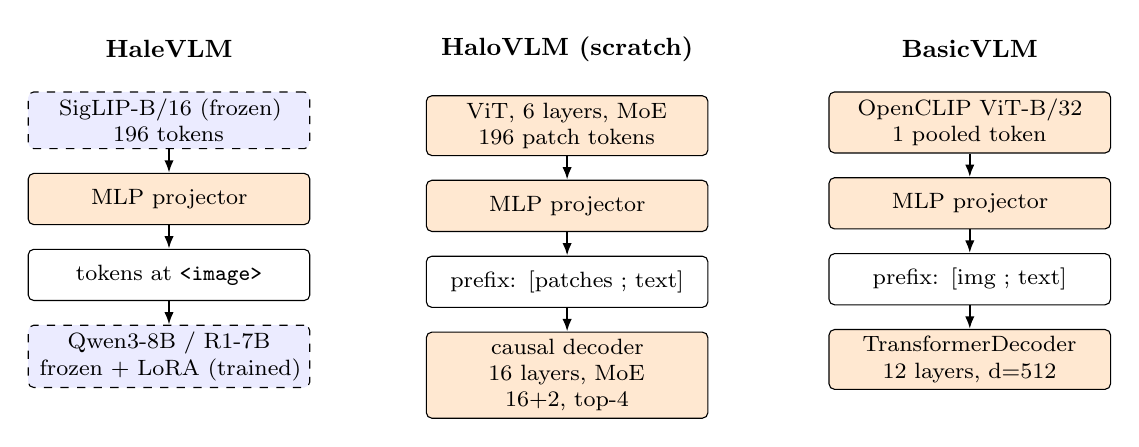
\begin{tikzpicture}[
  node distance=3mm and 4mm,
  box/.style={draw, rounded corners=2pt, align=center, font=\footnotesize, minimum height=6.5mm, inner sep=2.5pt, text width=34mm},
  fr/.style={box, fill=blue!8, dashed},
  tr/.style={box, fill=orange!18},
  hd/.style={font=\small\bfseries},
  arr/.style={-{Latex[length=1.6mm]}, thick}
]
\node[hd] (h1) {HaleVLM};
\node[fr, below=of h1] (a1) {SigLIP-B/16 (frozen)\\196 tokens};
\node[tr, below=of a1] (b1) {MLP projector};
\node[box, below=of b1] (c1) {tokens at \tok{image}};
\node[fr, below=of c1] (d1) {Qwen3-8B / R1-7B\\frozen + LoRA (trained)};
\draw[arr] (a1)--(b1); \draw[arr] (b1)--(c1); \draw[arr] (c1)--(d1);

\node[hd, right=24mm of h1] (h2) {HaloVLM (scratch)};
\node[tr, below=of h2] (a2) {ViT, 6 layers, MoE\\196 patch tokens};
\node[tr, below=of a2] (b2) {MLP projector};
\node[box, below=of b2] (c2) {prefix: [patches ; text]};
\node[tr, below=of c2] (d2) {causal decoder\\16 layers, MoE 16+2, top-4};
\draw[arr] (a2)--(b2); \draw[arr] (b2)--(c2); \draw[arr] (c2)--(d2);

\node[hd, right=24mm of h2] (h3) {BasicVLM};
\node[tr, below=of h3] (a3) {OpenCLIP ViT-B/32\\1 pooled token};
\node[tr, below=of a3] (b3) {MLP projector};
\node[box, below=of b3] (c3) {prefix: [img ; text]};
\node[tr, below=of c3] (d3) {TransformerDecoder\\12 layers, d=512};
\draw[arr] (a3)--(b3); \draw[arr] (b3)--(c3); \draw[arr] (c3)--(d3);
\end{tikzpicture}
\caption{The three model paths in Halo-VLM. Dashed boxes are frozen and orange boxes are
trained. The LLM in HaleVLM is frozen apart from its LoRA adapters.}
\label{fig:paths}
\end{figure}

\paragraph{HaleVLM (pretrained, parameter-efficient).} SigLIP-B/16~\cite{zhai2023siglip}
(or CLIP~\cite{radford2021clip}) produces 196 patch features that an MLP
($768\to2d\to d$, GELU) projects into the embedding space of a dense LLM:
Qwen3-8B~\cite{qwen3} or DeepSeek-R1-Distill-Qwen-7B~\cite{deepseekr1}. The projected tokens are
spliced into the sequence at the \tok{image} placeholder. The encoder and LLM are frozen,
and LoRA~\cite{hu2022lora} (rank 16, $\alpha=32$) is applied to the q, k, v, o, gate, up and
down projections. The trainer passes only the projector and adapter parameters to the
optimiser. This amounts to about 83.5M trainable parameters for Qwen3-8B and 71.6M for
R1-Distill-7B (computed from the backbone shapes), and the loss is the backbone's causal
LM loss.

\paragraph{HaloVLM (from scratch, MoE).} See \cref{sec:halo}.

\paragraph{BasicVLM (CLIP-prefix baseline).} An OpenCLIP~\cite{cherti2023openclip} ViT-B/32
pretrained on LAION-2B~\cite{schuhmann2022laion5b} (not frozen) produces one pooled image
embedding, which an MLP projects to $d=512$ and prefixes to the text embeddings. Sinusoidal
positions are added, and a 12-layer PyTorch \texttt{TransformerDecoder} (64 heads, FFN 1024,
37.9M parameters) runs with a causal target mask and key-padding mask. Having one visual
token makes this the cheapest possible fusion and a useful lower bound.

\Cref{tab:compare} summarises the differences.

\begin{table}[t]
\centering
\caption{Comparison of the three model paths.}
\label{tab:compare}
\small
\begin{tabular}{lccc}
\toprule
 & HaleVLM & HaloVLM & BasicVLM \\
\midrule
Vision encoder & SigLIP-B/16 (frozen) & ViT + MoE (scratch) & OpenCLIP ViT-B/32 (trained) \\
Visual tokens & 196 & 196 & 1 \\
Fusion & splice at \tok{image} & prefix & prefix \\
Language model & Qwen3-8B / R1-7B & 16-layer MoE decoder & 12-layer TransformerDecoder \\
Tokenizer & backbone's & BERT (30{,}522) & BERT (30{,}522) \\
Trained params & $\approx$72--84M (LoRA + proj.) & 431.5M (all) & all \\
Training backend & generic trainer & scratch trainer & scratch trainer \\
\bottomrule
\end{tabular}
\end{table}

\section{HaloVLM: A From-Scratch MoE VLM}
\label{sec:halo}

\paragraph{Vision encoder.} A $16\times16$ convolutional patch embedding turns a $224\times224$
image into 196 tokens of width $d=512$. Learned positions are added, and six pre-norm
transformer blocks (16 heads) follow, with a final LayerNorm~\cite{dosovitskiy2021vit}.

\paragraph{Decoder.} The projected patches are prefixed to the embedded caption tokens, and
learned absolute positions (up to 5{,}000) are added. The sequence is then processed by 16
causal pre-norm blocks with 32 heads. Every feed-forward layer in both the encoder and the
decoder is a DeepSeekMoE~\cite{dai2024deepseekmoe} layer: two shared SwiGLU~\cite{shazeer2020glu}
experts that every token uses, plus 16 routed experts, of which each token uses the top 4
under noisy gating~\cite{shazeer2017outrageously}. Expert hidden width is
$\mathrm{round}(1.2d)=614$.

\paragraph{Objective.} Captions are formatted as ``Describe the image'' followed by the
caption and a separator token, tokenised with BERT's WordPiece
vocabulary~\cite{devlin2019bert}, and converted to next-token targets by shifting left by
one. Padding is masked. The 196 image positions receive target $-100$, so the loss is pure
next-token cross-entropy on text conditioned on the visual prefix.

\begin{table}[t]
\centering
\caption{Measured parameter budget of HaloVLM (default \texttt{ScratchConfig}).}
\label{tab:halo}
\begin{tabular}{lrl}
\toprule
Module & Parameters & Notes \\
\midrule
Vision encoder & 108.8M & 6 layers, MoE 16 routed + 2 shared, top-4 \\
Image projector & 0.23M & $512\to128\to256\to512$ \\
Token embedding & 15.6M & BERT vocabulary, 30{,}522 \\
Position embedding & 2.6M & 5{,}000 positions \\
Decoder & 288.7M & 16 layers, 32 heads, same MoE \\
\quad active per token & $\approx$107.6M & attention + 2 shared + 4 routed experts \\
LM head & 15.6M & \\
\midrule
Total & 431.5M & \\
\bottomrule
\end{tabular}
\end{table}

\Cref{tab:halo} shows the budget. Because the vocabulary is small, 92\% of the parameters
sit in the vision and decoder MoE layers. Sparse routing keeps per-token compute at roughly
a third of the decoder's total parameter count.

\section{Library Design}
\label{sec:lib}

\paragraph{Configuration.} A run is a \texttt{VLMRunConfig}: strict \texttt{pydantic} sections that
reject unknown keys, loaded from YAML with \texttt{inherits:} deep-merging. The model section
holds \texttt{vision}, \texttt{llm} and \texttt{scratch} subsections and an \texttt{architecture}
field (\texttt{auto}, \texttt{hale}, \texttt{basic}, \texttt{halo\_moe}). With \texttt{auto}, the
architecture is derived from the variant name. The training section adds a \texttt{backend}
(\texttt{haleblocks} or \texttt{scratch}) and scratch-specific logging options.

\paragraph{Registries.} Models, losses, trainers, VLM datasets and VLA datasets are named
registries populated by decorators on import. \texttt{build\_vlm(cfg)} resolves the
architecture and instantiates the model. A variant's loss is registered under the same
name. External code can add a model without touching the library: the repository ships a
short example that registers a custom module.

\paragraph{Training and inference.} The Hale path uses a generic trainer whose optimiser sees
only trainable parameters. The scratch path uses a dedicated trainer with TensorBoard
logging of losses, gradient norms and weight statistics, prediction visualisations, and
token-by-token prediction videos. \texttt{VLMInference} provides greedy decoding, beam search
and streaming generation for scratch checkpoints.

\section{Data}
\label{sec:data}

The library registers all 19 datasets of the SmolVLM recipe~\cite{marafioti2025smolvlm}
by stage: vision (the Cauldron~\cite{laurencon2024matters}, Docmatix, MathWriting,
LLaVA-OneVision~\cite{li2024llavaonevision}), video (ten datasets including a text-SFT
share) and long context (five text corpora). SmolTalk is registered but disabled, because
the recipe found it harmful. A sequential mixer streams one dataset at a time up to a
per-dataset cap and warms up the next in the background. A second registry covers the
SmolVLA~\cite{shukor2025smolvla} robotics corpus (534 community, 2 simulation and 4
real-world datasets). A converter turns robot frames into VLM samples with
pretraining, fine-tuning or instruction-tuning prompts. The scratch models train on COCO
captions~\cite{lin2014coco} loaded through LAVIS~\cite{li2023lavis}, or on an overfit set for
smoke testing.

\section{Validation and Known Issues}

The library's test suite (unit, smoke and integration tests with tiny stand-in models)
passes on CPU: 29 tests pass and 2 are skipped. In reviewing the input pipeline we found
issues that should be fixed before reporting benchmark results with the HaleVLM path:
\begin{enumerate}
  \item \textbf{Image tokens overwrite text.} The prompt contains one \tok{image}
        placeholder, but the merge replaces \texttt{num\_image\_tokens} consecutive positions
        starting there, which drops the following $\texttt{num\_image\_tokens}-1$ text tokens.
        \emph{Fix:} expand the placeholder to \texttt{num\_image\_tokens} tokens during
        tokenisation, or insert rather than overwrite and extend \texttt{labels} with $-100$.
  \item \textbf{Supervision covers the prompt.} HaleVLM labels equal the input ids except
        padding. \emph{Fix:} mask non-assistant spans.
\end{enumerate}
The scratch HaloVLM ignores its attention mask and relies on the causal mask with
right-padding, which is correct for the provided collators but not for left-padded inputs.

\section{Experiments}

% TODO: add results only once produced by this library.
No benchmark results are reported in this version. The comparison the library is built for
is: all three paths trained on COCO captions with matched data and steps, evaluated with
standard captioning metrics; the effect of the number of visual tokens (1 vs.\ 196); dense
versus MoE layers in HaloVLM; and HaleVLM with each backbone on the SmolVLM vision stage.

\section{Conclusion}

Halo-VLM gives three very different VLM recipes a common home, from a frozen 8B LLM with
LoRA to a from-scratch MoE model to a one-token CLIP baseline. Shared configuration, data
and tooling make it possible to compare them on equal terms. We release it to make such
comparisons, and the ablations inside each regime, cheap to run.

\bibliographystyle{plainnat}
\bibliography{references}

\end{document}
